\documentclass[letterpaper,10pt,twocolumn]{article}

\usepackage[margin=0.75in]{geometry}
\usepackage{times}
\usepackage{helvet}
\usepackage{courier}
\usepackage{microtype}
\usepackage{graphicx}
\usepackage{amsmath,amssymb,amsthm}
\usepackage{booktabs}
\usepackage{array}
\usepackage{xcolor}
\usepackage{tikz}
\usepackage{url}
\usepackage{natbib}
\usepackage{enumitem}
\usepackage{caption}
\usepackage{algorithm}
\usepackage{algpseudocode}
\usetikzlibrary{arrows.meta,positioning,fit,calc,shapes.geometric}

\setlength{\pdfpagewidth}{8.5in}
\setlength{\pdfpageheight}{11in}
\setlength{\columnsep}{0.25in}
\emergencystretch=1.5em
\urlstyle{rm}
\def\UrlFont{\rm}
\frenchspacing

\newcommand{\safe}{\textsc{Safe}}
\newcommand{\cont}{\textsc{Continue}}
\newcommand{\abstain}{\textsc{Abstain}}
\newcommand{\pexp}{p_{\mathrm{exp}}}
\newcommand{\gexp}{G_{\mathrm{exp}}}
\newcommand{\supp}{\mathrm{support}}
\newcommand{\OmegaSR}{\Omega}

\newtheorem{proposition}{Proposition}

\title{Local Evidence Is Not Completion:\\ Evidence-Condition Geometry for Bounded Completion-Audit Workflows}
\author{Anonymous Submission}
\date{}

\begin{document}
\maketitle

\begin{abstract}
Bounded completion-audit workflows with declared source-route scopes often need
to decide whether a task is complete before the remaining workload is known.
Common stop signals, including no-new findings, agent agreement, stable
summaries, and self-reported completion, can be useful local evidence, but they
do not specify the conditions under which that evidence was produced. The key
question is not whether a workflow has stopped, but whether the evidence
condition under which it stopped can support the declared scope of the completion
claim. We study this certificate mismatch and introduce source-route
evidence-condition geometry as a runtime diagnostic. A source-route stratum
records both where the workflow searched and which audit route it applied. We
then define an evidence-condition controller that rejects \safe{} when the
current condition is too localized, repairs weak plausible strata, and returns
\safe{}, \cont{}, or \abstain{}. Across four bounded completion-audit tests,
homogeneous route reuse produces localized evidence conditions and would lead to
false certification if accepted as a scope-wide stop. Broader source-route
exposure improves completion eligibility, while an external \texttt{urllib3}
audit shows the key boundary: broad exposure is not sufficient for \safe{} when
residual evidence remains. The paper provides a diagnostic and control principle
for bounded audit completion, not a universal completion guarantee for open-world
agent workflows.
\end{abstract}

\section{Introduction}

This paper evaluates bounded completion-audit workflows with declared
source-route scopes. These are workflows whose intended evidence region is
bounded, such as a repository snapshot or document set, and whose completion
claim is stated over a declared set of sources and audit routes. Examples include
searching a repository snapshot for all instances of a behavior, auditing a
document set for policy exceptions, checking whether an implementation covers
declared failure-mode routes, or deciding whether a multi-agent audit has
exhausted useful evidence within its declared scope. Such workflows must
eventually stop. The difficulty is that the absence of newly found evidence is
not the same object as evidence that the intended bounded workload is complete.

The failure studied in this paper is \emph{certificate mismatch}. A workflow may
produce a plausible local stop signal: repeated scans return no new findings,
agents agree with each other, subtasks appear closed, or a summary becomes
stable. These signals are conditioned on the parts of the task that were searched
and on the routes by which they were searched. If the workflow repeatedly applies
the same route to the same subset of sources, a no-new signal may certify only
local exhaustion. It does not automatically support a global claim that the task
is complete over its intended scope.

Consider a code-audit workflow. Auditing a file for timeout behavior does not
certify that the same file has been audited for TLS behavior, exception behavior,
retry behavior, or cleanup behavior. The source may be familiar, the agents may
agree, and the workflow may have stopped finding timeout-related evidence; none
of that establishes that other routes over the same source have been exhausted.
The stop evidence is local in its evidence condition, while the completion claim
is global in scope.

We formalize this observation with \emph{evidence-condition geometry}. The basic
unit is a source-route stratum, consisting of a bounded evidence region and an
audit or search route. At runtime, the workflow accumulates exposure counts over
these strata. The normalized exposure distribution describes the condition under
which completion evidence was produced. When this distribution is localized,
stop evidence is locally conditioned. It may be useful, but it is not a global
completion certificate.

Based on this geometry, we define an evidence-condition controller. At a proposed
stop, the controller computes the source-route exposure condition, checks whether
the condition is broad enough to make the completion claim eligible for
certification, and triggers repair over weak plausible strata when necessary. The
controller is intentionally conservative: broad exposure gives completion
eligibility, not automatic safety. A \safe{} decision additionally requires that
repair or audit reveal no residual evidence. If residual evidence appears, the
controller outputs \cont{}; if budget is exhausted without a defensible
certificate, it outputs \abstain{}.

Our experiments evaluate this controller on four bounded completion-audit task
families: two generated scored tasks and two external real-repository audits with
pattern-defined oracles. These tasks are not presented as a benchmark for the
best item discovery policy. Instead, they test whether source-route exposure
localization diagnoses unsafe stop claims and whether a controller can avoid
accepting locally conditioned evidence as global completion proof.

This paper makes three contributions. First, it formulates false completion as a
certificate mismatch between the declared scope of a stop claim and the
source-route condition under which supporting evidence was produced. Second, it
introduces source-route exposure geometry and an evidence-condition controller
that separates completion eligibility from completion proof, repairing weak
plausible strata before accepting \safe{}. Third, it provides bounded audit
evaluation, including generated audits and external repository audits, showing
that homogeneous route reuse creates false certification risk while broader
source-route evidence improves eligibility without being sufficient for safety.

\begin{figure}[t]
\centering
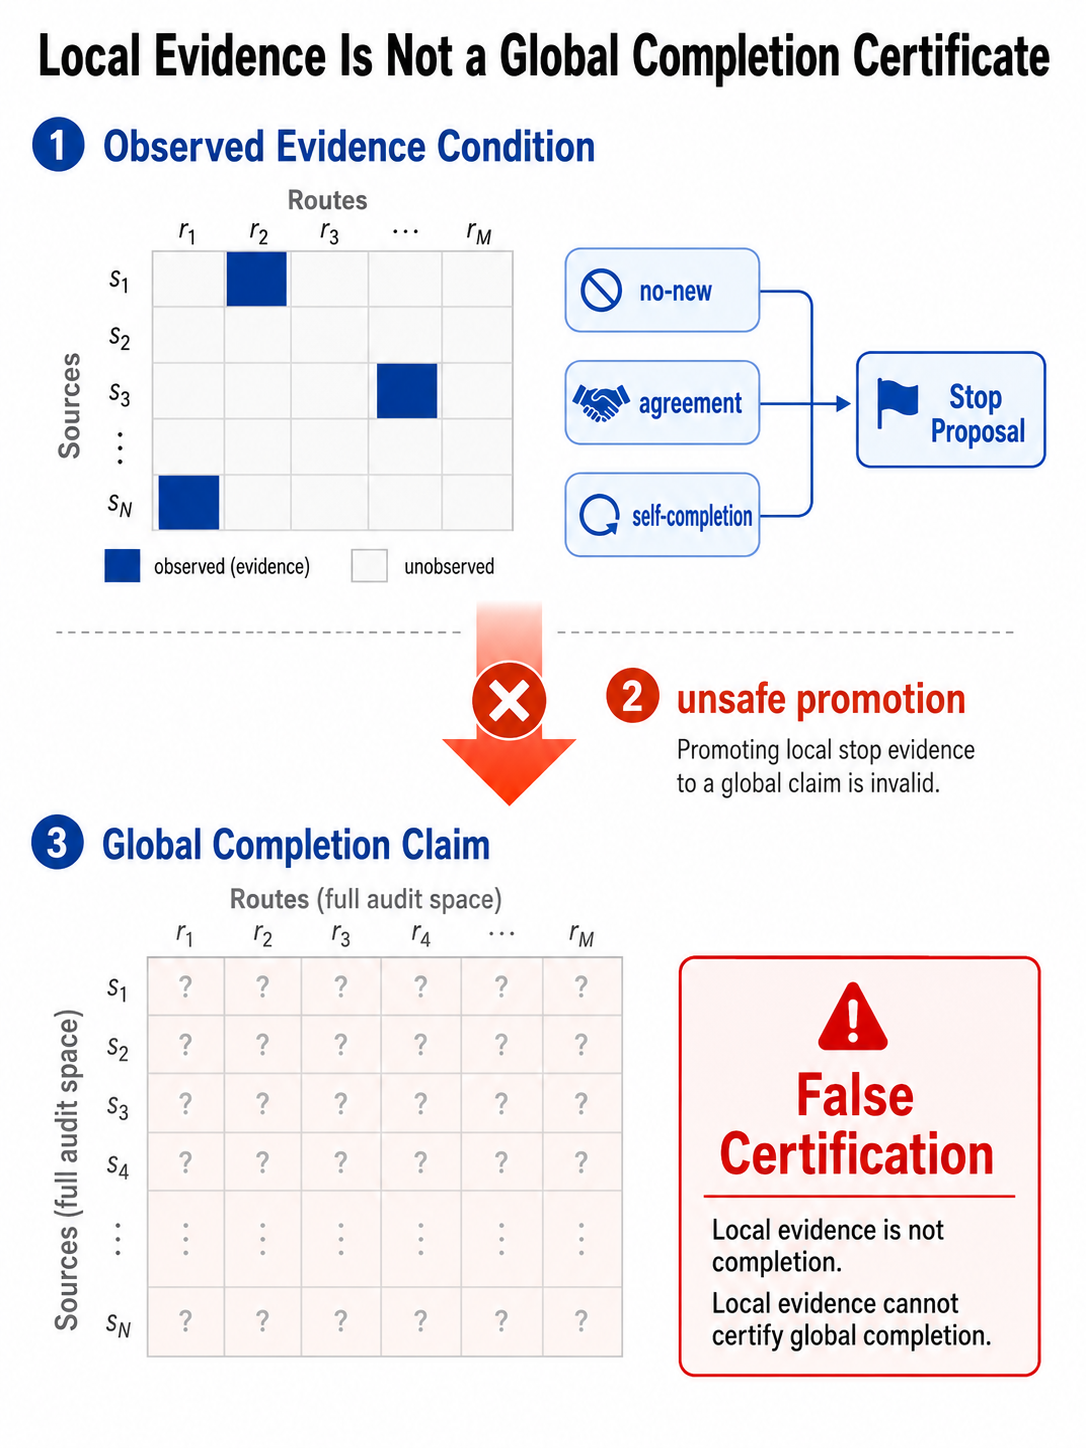
\includegraphics[width=\columnwidth]{figures/fig1.png}
\caption{Certificate mismatch from local stop evidence. A workflow may observe
no-new findings or agreement under localized source-route exposure. Such
evidence can support local exhaustion, but it does not by itself certify
completion over the intended source-route space. The evidence-condition
controller audits this condition before accepting \safe{}.}
\label{fig:mismatch}
\end{figure}

We deliberately do not claim that residual-potential is an optimal repair
method. It is one mechanism-aligned repair instance used to test whether weak
source-route regions can expose residual evidence. The main claim is about the
conditions under which completion evidence can support a stop decision.

\section{Related Work}

\paragraph{High-recall review, active search, and missing mass.}
Technology-assisted review and total-recall systems study how to retrieve nearly
all relevant items under review budgets
\citep{grossman2011technology,cormack2014evaluation,cormack2015multi,
cormack2016engineering,grossman2016trec,roegiest2015trec}, while active search
and active learning choose actions or examples to expose positives efficiently
\citep{lewis1994sequential,settles2009active,garnett2012bayesian,
attenberg2011beat}. Missing-mass and unseen-species estimators ask how much
probability mass remains unseen \citep{good1953population,
chao1984nonparametric,chao2014species}. Our scored subclasses use recall only
for post-hoc false-certification measurement. The controller does not observe
oracle totals, recall, or hidden missing mass; it observes the source-route
condition under which a stop claim was produced and whether repair reveals
residual evidence.

\paragraph{Agent workflows and verification.}
Tool-using, browser-assisted, multi-agent, and memory-based language agents
allocate work across tools, agents, searches, and intermediate states
\citep{yao2023react,schick2023toolformer,nakano2021webgpt,qin2024toolllm,
wu2023autogen,park2023generative,shinn2024reflexion,madaan2023selfrefine,
wang2024voyager}. Agent benchmarks and factual verification benchmarks evaluate
task success, tool use, factuality, or evidence support
\citep{yao2022alfworld,deng2024mind2web,zhou2024webarena,liu2024agentbench,
jimenez2024swebench,hendrycks2021measuring,liang2022holistic,
srivastava2023beyond,lin2022truthfulqa,thorne2018fever,gao2023rarr,
min2023factscore,schuster2021get}. Our question is narrower and precedes final
answer scoring: whether the evidence condition under which a workflow stopped is
broad enough for the scope of its completion claim.

\paragraph{Agreement, audit agents, and oversight.}
Ensembles, self-consistency, verifier-guided systems, and audit agents can
improve reliability \citep{dietterich2000ensemble,cobbe2021training,
wang2023selfconsistency}. Agreement is not useless, but it is unsafe as an
unconditioned completion certificate: agents may agree because they repeatedly
examined the same local region. Safety and oversight work studies broader
failure modes and scalable supervision \citep{amodei2016concrete,
christiano2017deep,irving2018ai,leike2018scalable,hendrycks2021unsolved}. This
paper targets a specific operational failure within that broader landscape: a
workflow may present a global completion certificate whose supporting evidence
was produced under a local source-route condition.

\section{Problem Setting}

We study bounded completion-audit workflows with unknown residual workload and
declared source-route scope. A workflow receives a task, allocates work across
agents or tools, gathers evidence under a finite budget, and must decide whether
the task is complete within that declared scope. Let
\[
W=(T,S,R,A,B),
\]
where \(T\) is the task, \(S\) is a set of sources, \(R\) is a set of routes,
\(A\) is the set of agents or tools, and \(B\) is a finite budget. A source is a
bounded evidence region, such as a file, module, document, source family, or
repository component. A route is an audit or search lens applied to a source.

At runtime, the workflow produces evidence events
\[
e_t=(a_t,x_t,r_t,u_t,o_t,c_t),
\]
where \(a_t\) is the agent or tool, \(x_t\in S\) is the source, \(r_t\in R\) is
the route, \(u_t\) is the action, \(o_t\) is the observation, and \(c_t\) is the
cost. Every evidence event is produced under a source-route condition. A
source-route stratum is \(s=(x,r)\), and the intended evidence-condition space is
\[
\OmegaSR=S\times R.
\]
The source-route space does not require the workflow to know all true missing
items in advance. It requires the intended audit scope to be defined: which
sources and routes are relevant to the completion claim.
This assumption is weaker than knowing the answer set and stronger than an
unbounded open-world search. It matches many practical audits: a system may know
which repositories, documents, modules, or evidence sources are in scope, and it
may know which audit routes are relevant, while still not knowing how many true
findings remain. The controller therefore evaluates the condition under which
evidence was gathered, not the unknown total workload itself.

A stop claim is a workflow assertion
\[
C_t:\quad T \text{ is complete over the intended workload scope.}
\]
A false certification occurs when the workflow accepts \safe{} for a stop claim
that is not supported by the evaluation oracle:
\[
\safe(C_t)=\mathrm{true},\qquad \mathrm{complete}(T)=\mathrm{false}.
\]
In item-discovery subclasses, this is operationalized as accepting \safe{} while
bounded-oracle recall is below the completion threshold. In broader completion
audits, it means accepting a global completion claim while relevant support,
contradiction, or unresolved evidence remains outside the evidence condition.
The oracle is used only for evaluation. It is not available to route assignment,
repair scoring, eligibility checks, or stop decisions.

\section{Evidence-Condition Geometry}

Let \(v_t(s)\) be the runtime-visible exposure count for source-route stratum
\(s\) up to time \(t\). Exposure may count visits, scans, route-specific audits,
tool calls, or other logged search actions. Define
\[
\pexp(t,s)=\frac{v_t(s)}{\sum_{s'\in\OmegaSR} v_t(s')}.
\]
This distribution is a point on the source-route coverage simplex. It describes
where and how completion evidence was produced.

We use two runtime summaries:
\[
\supp(t)=\frac{|\{s:v_t(s)>0\}|}{|\OmegaSR|},
\]
\[
\gexp(t)=\mathrm{Gini}(\{v_t(s):s\in\OmegaSR\}).
\]
These summaries are operational diagnostics, not universal laws. They summarize
whether the evidence condition is localized or broad enough to make a completion
certificate eligible for consideration.

\begin{proposition}[Local no-new evidence is not a global certificate]
Let \(U\subset \OmegaSR\) be a strict subset of the intended source-route space.
Suppose all evidence used to support a stop claim \(C_t\) is produced inside
\(U\), and suppose the workflow observes no-new evidence only for actions inside
\(U\). Then the no-new evidence can support local exhaustion over \(U\), but it
cannot by itself support global completion over \(\OmegaSR\).
\end{proposition}

\noindent\textit{Proof sketch.}
No-new evidence is conditioned on the source-route actions that were executed.
If no events are produced in \(\OmegaSR\setminus U\), the workflow has not
observed the absence of residual evidence in those unexposed strata. A world in
which \(U\) is exhausted and \(\OmegaSR\setminus U\) contains residual evidence
is observationally indistinguishable from a globally complete world under the
workflow's local evidence log. Therefore local no-new evidence rules out
additional findings only under the searched condition \(U\); without additional
assumptions about unsearched strata, it cannot rule out residual evidence in
\(\OmegaSR\setminus U\).

Source-only geometry is too coarse: auditing a file for timeout behavior does
not certify that TLS, retry, exception, or cleanup behavior has been audited in
that file. Source-route-action geometry is more detailed, but it is sensitive to
logging conventions and current experiments do not show a stable advantage over
source-route. Source-route is the default because it captures both where and how
evidence was produced while remaining interpretable and runtime-computable.
The geometry is thus a certificate diagnostic rather than a semantic theory of
all possible evidence. It asks whether the current log covers the intended
source-route space broadly enough for the proposed stop claim; it does not assert
that all routes are equally important or that support/Gini thresholds transfer
unchanged across domains.

\begin{figure*}[t]
\centering
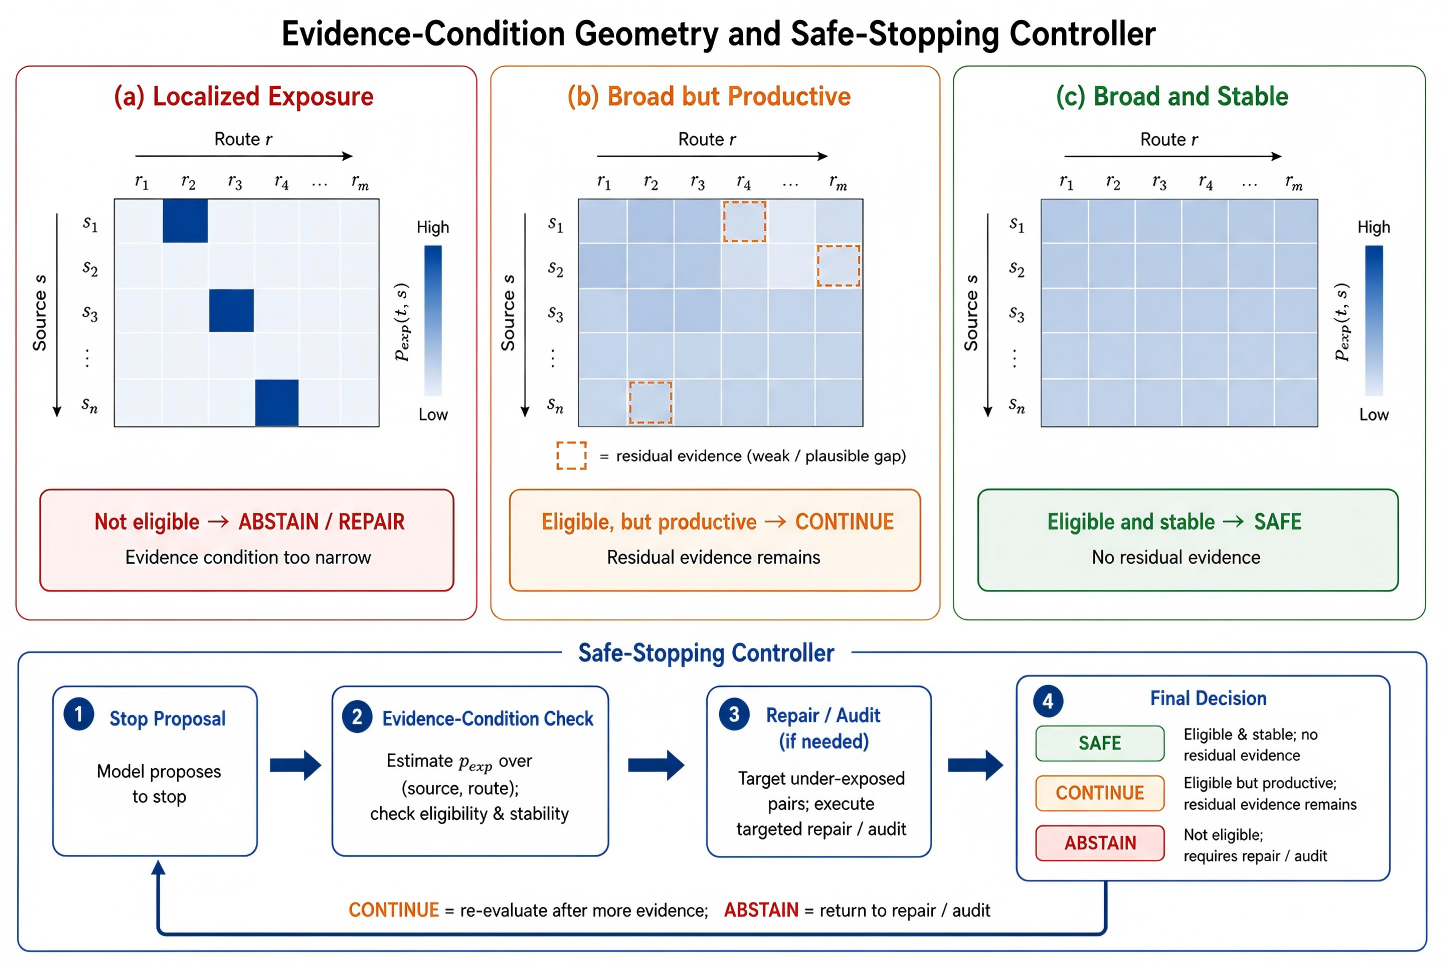
\includegraphics[width=0.78\textwidth]{figures/fig2-2.png}
\caption{Evidence-condition controller. The controller maps a runtime evidence
log to an exposure distribution over the intended source-route space. The
support/Gini check is an eligibility test, not a completion proof. If the
condition is localized or weak plausible gaps remain, the controller repairs or
continues. It returns \safe{} only when the evidence condition is broad and
repair or audit reveals no residual evidence.}
\label{fig:controller}
\end{figure*}

\section{Evidence-Condition Controller}

At a proposed stop, the controller checks whether the current evidence condition
can support the stop claim. Algorithm~\ref{alg:controller} makes the interface
explicit.

\begin{algorithm}[t]
\caption{Evidence-Condition Controller}
\label{alg:controller}
\begin{algorithmic}[1]
\Require log \(E_t\), space \(\OmegaSR\), claim \(C_t\), budget \(B\), thresholds
\(\tau_s,\tau_g\), repair rule \(\mathcal{R}\)
\Ensure decision in \(\{\safe{},\cont{},\abstain{}\}\)
\State Compute \(v_t(s)\), \(\pexp(t,s)\), \(\supp(t)\), and \(\gexp(t)\)
\State \(eligible \gets [\supp(t)\ge \tau_s \wedge \gexp(t)\le \tau_g]\)
\If{not \(eligible\) and \(B=0\)} \State \Return \abstain{} \EndIf
\If{not \(eligible\) or weak plausible gaps remain}
  \State Audit \(Q=\mathcal{R}(E_t,\OmegaSR,C_t)\) within \(B\)
  \If{residual evidence appears} \State \Return \cont{} \EndIf
  \State Recompute \(eligible\)
\EndIf
\If{\(eligible\) and no residual evidence appeared} \State \Return \safe{} \EndIf
\State \Return \abstain{}
\end{algorithmic}
\end{algorithm}

The eligibility check is not a completion proof. It is only a test of whether the
evidence condition is broad enough for a global stop claim to be considered. A
\safe{} decision additionally requires that repair or audit reveal no residual
evidence. In the current implementation, support and Gini thresholds instantiate
an operational eligibility check; these thresholds are not claimed as universal
laws.
This separation is important for reviewer interpretation. A localized no-new
signal should normally trigger repair or continuation, but a broad exposure
state is still only a license to ask the stronger question: do weak plausible
gaps remain productive under additional audit? The controller therefore prevents
the common shortcut in which broad coverage is treated as direct proof of global
completion.

\paragraph{Residual-potential repair.}
The repair instance used in the experiments is
\[
\mathrm{priority}(s)=\mathrm{under\_exposure}(s)\cdot
\mathrm{runtime\_potential}(s).
\]
The under-exposure term gives priority to weak parts of the current completion
certificate. The runtime-potential term uses visible information such as source
text, route names, source size, route match counts, or non-oracle ledger signals.
It is not allowed to use oracle labels, oracle totals, oracle missing mass,
undiscovered true item counts, post-hoc recall, or scorer-visible target
distributions. Residual-potential is a mechanism-aligned repair instance, not an
optimal active-search algorithm.

\section{Experiments}

The experiments are not a discovery benchmark. They are controlled
completion-audit tests designed to check whether stop evidence is sufficient to
support a completion claim under a declared source-route scope.

We organize experiments around four research questions. RQ1 asks whether
localized source-route evidence creates false certification risk. RQ2 asks
whether broad exposure provides eligibility rather than completion proof. RQ3
asks whether the evidence-condition controller reduces unsafe stop decisions.
RQ4 asks where residual-potential differs from high-potential repair.

\paragraph{Tasks.}
\texttt{policy\_docset\_v1} is a generated policy document set with four
sources covering access control, data handling, release process, and audit
exceptions. Its routes are obligation, exception, deadline, and prohibition; the
hidden oracle contains 24 policy clauses. \texttt{code\_repo\_v1} is a generated
bounded code repository with authentication, payment, storage, and API-client
sources. Its routes are compatibility, security, and resilience; the hidden
oracle contains 20 code-risk items.

\texttt{requests} is an external real-repository audit over six files from a
local installed snapshot of the Python package: adapters, API, authentication,
models, sessions, and utilities. Its routes are TLS, timeout, exception, and
compatibility. \texttt{urllib3} is an external real-repository audit over
connection, connection-pool, pool-manager, response, retry, and timeout sources.
Its routes are timeout, retry, TLS, exception, and cleanup, giving 30 intended
source-route strata. External oracles are pattern-defined from frozen snapshots:
stronger than generated toys, weaker than human-annotated completion-audit
benchmarks.

\paragraph{Workflow conditions.}
Homogeneous route reuse assigns multiple agents to the same route across
sources. The reused routes are obligation for \texttt{policy\_docset\_v1},
compatibility for \texttt{code\_repo\_v1}, and timeout for the two external
repository audits.
Route-partitioned audit assigns agents to different routes over the same source
set. \texttt{urllib3} additionally includes an \texttt{extended\_audit}
condition covering all five routes.

\paragraph{Seeds, budgets, thresholds, and cost.}
Generated-task first-pass challengers used a target budget of 4 strata; method
validation reran generated-task challengers for 200 seeds. \texttt{requests}
challengers used 200 seeds and a budget of 4 strata. \texttt{urllib3}
challengers used 200 seeds and a budget of 5 strata. The external controller
validation uses \(\tau_s=0.75\) and \(\tau_g=0.70\). A 0.90 recall threshold is
used only for bounded-oracle evaluation of false certification and is not visible
to the controller. We separate original workflow cost from post-hoc audit cost:
repair cost and confirmation-audit cost count only the additional scanned source
lines plus extraction events after a stop state is fixed. Thus safe-state
validation can have repair gain \(0\) but positive cost: the extra probes are
confirmation audits that verify no additional route-level evidence appears. For
each seed, route assignment, repair ordering, and challenger choice are fixed
before oracle scoring. This makes the reported false-certification and repair
measurements post-hoc evaluations of fixed trajectories rather than inputs to
the controller.

\begin{table*}[t]
\centering
\caption{Experimental coverage. The main evaluation combines generated audits,
external repository audits, seeded repair/controller validation, and simulation
stress tests. Pattern-defined external oracles are used only for post-hoc
scoring.}
\label{tab:coverage}
\resizebox{\textwidth}{!}{%
\begin{tabular}{llrrrrl}
\toprule
Study & Role & Sources & Routes/strata & Oracle items & Runs/seeds & Main measurement \\
\midrule
\texttt{policy\_docset\_v1} & generated audit & 4 & 4/16 & 24 & 200/challenger & false certification, repair gain \\
\texttt{code\_repo\_v1} & generated audit & 4 & 3/12 & 20 & 200/challenger & false certification, repair gain \\
\texttt{requests} & external repo audit & 6 & 4/24 & 298 & 200/challenger & controller validation \\
\texttt{urllib3} & external repo audit & 6 & 5/30 & 699 & 200/challenger & boundary validation \\
Controlled geometry & simulation stress test & -- & variable & synthetic & 2160 runs & metric screening \\
Exposure localization & simulation stress test & -- & 18/30/42 & synthetic & 2700 runs & exposure vs. discovery localization \\
\bottomrule
\end{tabular}}
\end{table*}

Table~\ref{tab:coverage} summarizes the amount of evidence behind the empirical
claims. The four task families supply bounded completion-audit cases with
withheld or post-hoc oracles. The simulation stress tests are not used as main
task results; they check whether the geometry variables behave consistently
under larger controlled sweeps and whether the diagnostic is an artifact of a
single task family. Leakage-control details are reported in the anonymous
supplementary material; runtime decisions use visible logs and source text, not
oracle labels, oracle totals, post-hoc recall, or undiscovered true-item counts.

\section{Results}

\paragraph{RQ1: Localized evidence creates false certification risk.}
Figure~\ref{fig:main_results} reports the main diagnostic. Across all four tasks,
homogeneous route reuse produces localized evidence conditions and would cause
false certification if accepted as \safe{}. The result supports the diagnostic
claim: the false stop is not merely an item-recovery failure; it is a certificate
mismatch between local evidence and a global completion claim.
The finding is also consistent with controlled sweeps: in the 2160-run geometry
stress test, homogeneous and prompt-diverse local conditions have false-stop
rates of \(1.000\), while route-partitioned and extended audits reduce the rate
to \(0.637\) and \(0.546\), respectively. In the 2700-run exposure-localization
stress test, homogeneous and prompt-diverse conditions again remain near
complete false-stop failure (\(0.998\) and \(1.000\)).

\begin{figure*}[t]
\centering

\includegraphics[width=\textwidth]{figures/main_results_overview.pdf}
\caption{Main diagnostic and ablation. Left: homogeneous base states have low
source-route support; broader audits increase support. Middle: source-only
support is full in homogeneous runs, but source-route support remains localized,
exposing the route-level certificate mismatch. Right: \texttt{urllib3} is the
boundary case: route-partitioned audit is broad but incomplete, while the
extended audit reaches completion. Dashed lines mark the operational support and
recall thresholds used for evaluation.}
\label{fig:main_results}
\end{figure*}

\paragraph{RQ2: Broad exposure is eligibility, not proof.}
Route-partitioned evidence improves completion eligibility in all tasks, but it
does not always justify \safe{}. The \texttt{urllib3} row is the boundary case.
Route-partitioned exposure is broad enough to be geometry-eligible, but
bounded-oracle recall is below threshold and repair/audit remains productive.
The controller returns \cont{}, not \safe{}. The extended \texttt{urllib3} audit
reaches support \(1.000\), recall \(1.000\), and \safe{}.
This boundary is important because it prevents a different shortcut: replacing
local-stop acceptance with automatic acceptance of broad exposure. The
\texttt{urllib3} condition has 24 of 30 source-route strata exposed and 584 of
699 oracle items found, but weak plausible gaps remain and additional audit
finds residual evidence.

The middle panel of Figure~\ref{fig:main_results} gives the mechanism ablation
behind this claim. In the homogeneous runs, every task touches all source files,
so a source-only controller would see full support. Yet the same states have low
source-route support, high concentration, and sub-threshold bounded-oracle
recall. Source-only exposure therefore cannot detect the route-level mismatch:
auditing a file for timeout evidence does not certify TLS, retry, exception, or
cleanup routes in that file.

A scalar singleton/Chao-style proxy is included only as a negative control in
the supplementary tables. It summarizes item-count sparsity but does not encode
where evidence was gathered, so it cannot identify the route-level certificate
mismatch between a local no-new signal and a source-route completion claim.

\paragraph{RQ3: The controller reduces unsafe stops without merely refusing to stop.}
A naive controller that accepts local stop signals would falsely certify all four
homogeneous conditions. The evidence-condition controller rejects these stops
because the evidence condition is localized. It also avoids the trivial
``never stop'' solution: it returns \safe{} for the two generated tasks and for
\texttt{requests} under broad complete conditions, and reserves \safe{} for the
extended \texttt{urllib3} audit rather than the broad-but-incomplete
route-partitioned condition.
Across the two external repository controller validations, all seeded
repair/controller trials have zero false-certification rate after the controller
is applied: six \texttt{requests} challenger policies and five \texttt{urllib3}
challenger policies, each evaluated with 200 seeds. These trials do not
make the controller complete; they show that the implemented decision rule
rejects the unsafe local stops while still allowing \safe{} when the external
audit state is broad and nonproductive.
Figure~\ref{fig:controller_decisions} expands this accounting. Seeded repair
states are oracle-unsafe and mostly return \cont{} because repair remains
productive. Seeded safe states check the opposite failure mode: starting from
oracle-safe complete states, the controller remains \safe{} across 6000
order/budget perturbations. Both sides have FCR \(0\); safe-state coverage is
\(1\). The controller is therefore not a never-stop rule: it rejects unsafe
productive states without becoming over-conservative once the source-route
evidence condition matches the completion claim.

\begin{figure}[t]
\centering

\includegraphics[width=\columnwidth]{figures/controller_decision_matrix.pdf}
\caption{Controller decision accounting for external validations. Unsafe repair
states have 0\% \safe{} decisions, while safe complete states have 100\%
\safe{} decisions under order/budget perturbations. Oracle-safe and
oracle-unsafe denominators are used only for evaluation.}
\label{fig:controller_decisions}
\end{figure}

\paragraph{RQ4: Residual-potential is useful but bounded.}
Figure~\ref{fig:repair_sensitivity} summarizes the repair boundary.
Residual-potential
provides positive repair evidence but is not proven optimal. On \texttt{requests},
residual-potential and high-potential are identical at source-route granularity.
On \texttt{urllib3}, residual-potential recovers more total new evidence, but
high-potential is similar or slightly better in cost-normalized evidence. The
correct conclusion is that residual-potential is a mechanism-aligned repair
instance that can expose residual evidence, not an optimal active-search method.
The figure reports mean and 95\% confidence intervals for repair gain; where
policies overlap, the restrained reading is that the probe is informative, not
that one search policy dominates in a stable way.
This bounded conclusion is reinforced by metric screening. In the 2160-run
controlled-geometry study, coverage Gini is the strongest single diagnostic
(AUROC \(0.995\)), while the more elaborate compound risk quantity is weaker
(AUROC \(0.831\)). A leave-world-out check over three synthetic worlds keeps
coverage Gini stable (mean AUROC \(0.996\), minimum \(0.994\)). In the
2700-run exposure-localization study, exposure and discovery Gini are both
predictive (AUROC \(0.845\)), which supports the broader localization argument
without overclaiming that residual-potential is uniquely optimal.

\begin{figure}[t]
\centering

\includegraphics[width=\columnwidth]{figures/repair_sensitivity_summary.pdf}
\caption{Repair gain for residual-potential, high-potential, and random probes
with 95\% confidence intervals. Sensitivity details are reported in the
supplementary material.}
\label{fig:repair_sensitivity}
\end{figure}

\paragraph{Sensitivity and audit checks.}
Sensitivity details are moved to the supplementary material. Threshold and
budget sweeps over the external controller validations scan
\(\tau_s \in \{0.50,0.60,0.70,0.75,0.80,0.90\}\),
\(\tau_g \in \{0.50,0.60,0.70,0.80,0.90\}\), and repair budgets
\(\{1,2,4,6,8\}\). These sweeps mainly test unsafe productive states; changing
thresholds and budgets changes the \safe{}/\cont{}/\abstain{} mixture and repair
cost without creating false certifications. The seeded safe-state rows in
Figure~\ref{fig:controller_decisions} complement this by testing completed
oracle-safe states. Across threshold settings, \texttt{requests} has SAFE-rate
range \(0.000\)--\(0.000\), CONTINUE-rate range \(0.995\)--\(1.000\), and max FCR
\(0\); \texttt{urllib3} has SAFE-rate range \(0.000\)--\(0.000\),
CONTINUE-rate range \(0.990\)--\(1.000\), and max FCR \(0\). Budget sweeps keep
max FCR \(0\) while moving abstention up to \(0.365\) for \texttt{requests} and
\(0.360\) for \texttt{urllib3}. Oracle construction, scalar negative controls,
route-match consistency checks, workflow-shape/interface validation, leakage
controls, and regex examples are reported in the anonymous supplementary
material rather than used as main effectiveness evidence.

\section{Discussion and Validity}

The controller certifies a relationship between a stop claim and the evidence
condition that produced its support. It does not certify that the world contains
no further facts, that all future searches would fail, or that source-route is
the only possible abstraction. This distinction separates the paper from
total-recall and active-search optimization: recall is used only for post-hoc
false-certification measurement, while the runtime decision uses exposure,
eligibility, and repair outcomes. Multi-agent agreement is likewise not rejected
as useless; it is rejected only as an unconditioned completion certificate.

The main internal threat is leakage from the hidden oracle into repair or stop
decisions. The protocol constructs oracles offline, freezes trajectories before
scoring, and restricts runtime features to visible logs, source-route
identifiers, source text, lexical match counts, and non-oracle ledger signals.
Thresholds are operational test points, not learned universal constants.
Support and Gini measure exposure breadth and concentration rather than semantic
adequacy; domains with unequal route importance should declare weights or route
priorities before execution.

The experiments cover generated document/code audits and two real-repository
audits with pattern-defined oracles. This is broader than a toy-only validation
but narrower than a human-annotated benchmark of completion claims. The strongest
external claim is therefore limited: local source-route evidence can create false
completion certificates, and an evidence-condition controller can prevent this
class of unsafe stop in bounded audit settings. The paper does not claim
universal open-world completeness or optimal repair search.

\section{Limitations and Supplement}

The current evidence supports a diagnostic and controller in bounded
completion-audit subclasses. External oracles are pattern-defined rather than
human annotated; support/Gini thresholds are operational; source-route strata are
task-designed; and residual-potential is not proven optimal. The anonymous
supplementary material records reproducibility details that are not main
effectiveness evidence: the scalar negative control, external oracle
construction summary, workflow-shape/interface pilot, seeded safe-state
breakdown, route-match consistency sanity check, leakage-control matrix, and
route-wise pattern examples. A future claim-verification audit with support,
contradiction, exception-path, configuration-default, and scope-boundary routes
would test the same certificate-mismatch principle beyond item-discovery audits.

\section{Conclusion}

This paper studies completion decisions in bounded completion-audit workflows
with declared source-route scopes and unknown residual workload. The central
observation is simple but consequential: local evidence does not automatically
support a scope-wide completion claim. Stop signals such as no-new findings,
agreement, or stable summaries are conditioned on where and how the workflow
searched.

Source-route evidence-condition geometry makes this conditioning explicit. The
evidence-condition controller uses that geometry to reject unsafe local stops,
repair weak plausible strata, and reserve \safe{} for cases where the evidence
condition is broad and no residual evidence appears. Across generated and
external bounded audits, homogeneous route reuse consistently creates false
certification risk, while broader source-route exposure improves completion
eligibility without being sufficient by itself. The main contribution is not a
claim that a particular repair heuristic is optimal. It is a diagnostic and
control principle: completion certificates should be judged by the evidence
condition that produced them.

\bibliographystyle{plainnat}
\bibliography{references}

\section*{AAAI Reproducibility Checklist}

This paper includes computational experiments. The bounded scope, assumptions,
metrics, thresholds, and controller rule are described in the main text; the
supplement records script entry points, seeds, data/log formats, oracle fields,
figure-generation commands, and software environment. Randomness is controlled
by fixed seed sets before oracle scoring. The evaluation uses generated audits,
frozen repository snapshots, and pattern-defined oracles; oracle labels, oracle
totals, post-hoc recall, and undiscovered true-item counts are used only for
post-hoc scoring. Reported runs include 200-seed challenger validations for each
main task family, 6000 safe-state perturbations, 2160 controlled-geometry stress
runs, and 2700 exposure-localization stress runs. Variation is reported with
95\% confidence intervals for repair gains and with threshold/budget sweep
ranges in the supplementary material. The implementation and generated
artifacts are organized as a code/data supplement for anonymous review and can be
released on publication.

\end{document}
